\documentclass[12pt, letterpaper]{article}
\usepackage[utf8]{inputenc}
\usepackage[spanish]{babel}
\usepackage{amsmath, amssymb}
\usepackage{graphicx}
\usepackage{hyperref}
\usepackage{geometry}
\usepackage{fancyhdr}
\usepackage{setspace}

% Configuración de márgenes
\geometry{top=2.5cm, bottom=2.5cm, left=3cm, right=2.5cm}

% Configuración de encabezado y pie
\pagestyle{fancy}
\fancyhf{}
\renewcommand{\headrulewidth}{0pt}

\begin{document}

% ================================
% PORTADA (Página 1 - sin número)
% ================================
\begin{titlepage}
    \centering
    \vspace*{2cm}
    
    {\LARGE \textbf{Desgaste en superficies: representación de abolladuras}}\\[0.5cm]
    
    {\large \textbf{Alejandro Caicedo Caicedo}}\\
    {\large \textbf{Simón Díaz Monroy}}\\[0.3cm]
    
    \textit{Pontificia Universidad Javeriana}\\
    \texttt{caicedo\_alejandro@javeriana.edu.co}\\
    \texttt{simondiaz@javeriana.edu.co}\\[2cm]
    
    {\large \textbf{Fecha:} \today}\\[1cm]
    
    \vfill
\end{titlepage}

% ================================
% ÍNDICE (Página 2 - numeración romana)
% ================================
\newpage
\setcounter{page}{2}
\pagenumbering{roman}
\tableofcontents
\thispagestyle{empty}

% ================================
% CONTENIDO PRINCIPAL (Página 3 en adelante - numeración arábiga)
% ================================
\newpage
\setcounter{page}{1}
\pagenumbering{arabic}

% Activar encabezado para el resto del documento
\pagestyle{fancy}
\fancyhf{}
\cfoot{\thepage}

% ================================
% SECCIONES SOLICITADAS
% ================================
\section{Análisis del Problema}
El problema planteado consiste en modificar una superficie dada \(S\) para representar un conjunto de abolladuras \(D\). Cada abolladura se define sobre un subconjunto de áreas \(A\), especificando un círculo dentro de \(A\) y un valor de fuerza \(I \in [0,1]\). La solución requiere triangular la nube de puntos de \(S\), identificar los puntos que caen dentro del círculo de cada abolladura y aplicar un desgaste gradual, de modo que los puntos más cercanos al centro del círculo presenten una deformación más pronunciada, simulando así el efecto de una hendidura en la superficie.

\section{Marco teórico}
\subsection{Funciones de base radial}

Para reconstruir una función continua que represente el fenómeno en toda la superficie, se requiere una técnica de aproximación que sea que no dependa de una malla regular.

Las funciones de base radial (Radial Basis Functions, RBF) constituyen una de las herramientas más utilizadas para la aproximación de funciones multivariables a partir de datos dispersos. Su principal ventaja radica en que el aproximante se expresa como una combinación lineal de términos radiales centrados en cada punto de dato, lo que permite trabajar directamente con nubes de puntos sin necesidad de estructuras topológicas adicionales. Además, las RBF ofrecen rápida convergencia y buena precisión a la función objetivo, propiedades que las hacen adecuadas para aplicaciones en gráficos por computadora, reconstrucción de superficies y, como se mostrará en este trabajo, para la simulación de desgaste mediante abolladuras.

\paragraph{Esquema de aproximación.}
Sea \(f: \mathbb{R}^n \to \mathbb{R}\) una función que se conoce únicamente en un conjunto de \(m\) puntos distintos \(\mathbf{x}_1, \mathbf{x}_2, \dots, \mathbf{x}_m \in \mathbb{R}^n\), con valores correspondientes \(f(\mathbf{x}_1), f(\mathbf{x}_2), \dots, f(\mathbf{x}_m)\). El método de funciones de base radial construye un aproximante \(s: \mathbb{R}^n \to \mathbb{R}\) de la forma:
\[
s(\mathbf{x}) = \sum_{j=1}^{m} \lambda_j \, \phi\bigl(\|\mathbf{x} - \mathbf{x}_j\|\bigr), \qquad \mathbf{x} \in \mathbb{R}^n, \tag{1}
\]
donde:
\begin{itemize}
    \item \(\mathbf{x}_j\) son los puntos de datos (centros de las RBF), en los cuales se conoce el valor de \(f\).
    \item \(\mathbf{x}\) es una variable independiente en la que se evaluará el aproximante.
    \item \(\phi: \mathbb{R}_{\ge 0} \to \mathbb{R}\) es una función univariable, normalmente continua, denominada función de base radial. Su argumento es la distancia radial desde \(\mathbf{x}\) hasta cada centro.
    \item \(\|\cdot\|\) denota la norma euclídea en \(\mathbb{R}^n\).
    \item \(\lambda_j \in \mathbb{R}\) son coeficientes escalares que ponderan la contribución de cada centro.
\end{itemize}

En el caso general de interpolación, los coeficientes \(\lambda_j\) se determinan resolviendo un sistema lineal. Sin embargo, para este proyecto se adopta una versión simplificada que resulta suficiente para modelar abolladuras independientes: cada coeficiente \(\lambda_j\) se toma directamente proporcional al valor conocido \(f(\mathbf{x}_j)\). Es decir,
\[
\lambda_j = c \cdot f(\mathbf{x}_j),
\]
donde \(c\) es una constante de escala (por ejemplo, una constante de flexibilidad de la superficie). De esta manera, el aproximante queda expresado como:
\[
s(\mathbf{x}) = \sum_{j=1}^{m} c \, f(\mathbf{x}_j) \; \phi\bigl(\|\mathbf{x} - \mathbf{x}_j\|\bigr).
\]
Esta formulación evita la resolución de sistemas lineales.

\paragraph{Tipos de funciones de base radial.}

Existen diversas funciones de base radial que pueden utilizarse en el esquema de aproximación. Las más comunes se enumeran a continuación, donde \(r = \|\mathbf{x} - \mathbf{x}_j\|\) y \(\varepsilon > 0\) es un parámetro de forma que controla la extensión radial.

\begin{itemize}
    \item \textbf{Gaussiana}: 
    \[
    \phi(r) = e^{-(\varepsilon r)^2}
    \]

    \item \textbf{Multicuádrica (Multiquadric)}: 
    \[
    \phi(r) = \sqrt{1 + (\varepsilon r)^2}
    \]

    \item \textbf{Multicuádrica inversa (Inverse Multiquadric)}: 
    \[
    \phi(r) = \frac{1}{\sqrt{1 + (\varepsilon r)^2}}
    \]

    \item \textbf{Thin plate spline}: 
    \[
    \phi(r) = r^2 \ln(r)
    \]

    \item \textbf{Cúbica}: 
    \[
    \phi(r) = r^3
    \]

    \item \textbf{Lineal}: 
    \[
    \phi(r) = r
    \]
\end{itemize}

\paragraph{Funciones de Wendland (soporte compacto)}
Una familia de funciones de base radial con soporte compacto. Estas funciones son polinomios por tramos en el intervalo \([0, R]\) y se construyen para ser positivas definidas en \(\mathbb{R}^d\) y con un grado de suavidad \(C^{2k}\) controlado. Se denotan por \(\phi_{d,k}(r)\), donde:

\begin{itemize}
    \item \(d\) es la dimensión del espacio euclídeo donde se trabaja (por ejemplo, \(d=2\) o \(d=3\)).
    \item \(k\) es un parámetro entero no negativo que determina la suavidad: la función resultante es \(C^{2k}\) en \(r=0\) y en \(r=R\).
\end{itemize}

La expresión general para \(\phi_{d,k}(r)\) se obtiene mediante integración repetida a partir de una función generadora. En la práctica, se utilizan las formas explícitas para combinaciones concretas de \(d\) y \(k\).

\paragraph{Caso particular \(\phi_{3,1}\)}
Para el espacio tridimensional (\(d=3\)) y con el menor grado de suavidad que garantiza continuidad hasta la primera derivada (\(k=1\)), se obtiene la función:
\[
\phi_{3,1}(r) = \left(1 - \frac{r}{R}\right)_+^4 \left(4\frac{r}{R} + 1\right),
\]
donde \((\cdot)_+ = \max(0,\cdot)\) y \(R>0\) es el radio de soporte. El subíndice \(3,1\) indica que la función es adecuada para \(\mathbb{R}^3\) y proporciona una suavidad \(C^2\).

\paragraph{Restricción espacial y selección de puntos}
Para el problema planteado, cada abolladura afecta únicamente a los puntos de la superficie que se encuentran dentro de un círculo de radio \(R_i\) (definido por su área de cobertura). Para cumplir esta restricción, el algoritmo puede implementar dos estrategias complementarias:

\begin{enumerate}
    \item \textbf{Uso de una función de base radial con soporte compacto}.  
    Funciones como la de Wendland son idénticamente nulas para \(r \ge R_i\). Al emplearlas en la ecuación (1), la deformación se anula fuera del círculo.

    \item \textbf{Uso de una función de soporte global con filtrado explícito}.  
    Funciones como la gaussiana o la multicuádrica toman valores positivos para cualquier distancia, aunque sean muy pequeños. En este caso, el algoritmo evalúa la deformación solo para aquellos puntos cuya distancia al centro de la abolladura sea menor que \(R_i\); los puntos externos no se modifican. Esta aproximación permite conservar la suavidad de la función dentro del radio de influencia.
\end{enumerate}

\section{Diseño del algoritmo}

\subsection{Entradas}
El algoritmo recibe los siguientes elementos:
\begin{itemize}
    \item \(P = \{p \in \mathbb{R}^3\}\), nube de puntos que representa la superficie original \(S\).
    \item \(D\): conjunto de abolladuras \(D = \{d_1, d_2, \dots, d_M\}\). Cada abolladura \(d_i\) se define por:
        \begin{itemize}
            \item centro \(\mathbf{c}_i = (x_i, y_i)\),
            \item radio \(R_i\) (circunferencia que delimita el área de influencia),
            \item intensidad \(I_i \in [0,1]\) (profundidad máxima en el centro).
        \end{itemize}
    \item \(\phi\): tipo de función de base radial a utilizar. Se especifica mediante una categoría o bandera (ej. ``gaussiana'', ``wendland'', ``multicuádrica''). La implementación concreta de cada fórmula se detalla en la sección de implementación.
\end{itemize}

\subsection{Salidas}
El algoritmo produce:
\begin{itemize}
    \item \(P'\): la nube de puntos \(P\) con las coordenadas \(z\) modificadas según las abolladuras.
    \item Una triangulación (estructura de media arista) que representa la conectividad de la malla.
\end{itemize}

\subsection{Estructuras de datos}
Para representar la triangulación de la superficie se emplea una estructura de datos de media arista (half‑edge).

\section{Descripción del procedimiento}

El algoritmo se divide en dos componentes principales.

\subsection{Triangulación y selección de zonas de abolladura}

\begin{enumerate}
    \item \textbf{Construcción de la triangulación.}  
    Se toma la proyección \((x, y)\) de todos los puntos de \(P\) y se calcula su triangulación de Delaunay. La conectividad resultante se almacena en la estructura de media arista.

    \item \textbf{Selección de puntos por abolladura.}  
    Para cada abolladura \(d_i \in D\):
    \begin{itemize}
        \item Se calcula la distancia euclídea desde su centro \(\mathbf{c}_i\) a cada punto \(\mathbf{p} \in P\).
        \item Se recolectan todos los puntos que cumplen \(\|\mathbf{p}_{xy} - \mathbf{c}_i\| < R_i\).
        \item Estos puntos conforman el conjunto \(A_i \subseteq P\) (zona afectada por la abolladura \(i\)).
    \end{itemize}

    \item \textbf{Retorno.}  
    Se entrega la triangulación de Delaunay y la colección de conjuntos \\ \(\{A_1, A_2, \dots, A_M\}\).
\end{enumerate}

\subsection{Deformación mediante funciones de base radial}

\begin{enumerate}
    \item \textbf{Inicialización.}  
    Para cada punto \(\mathbf{p} \in P\), se establece \(\Delta z(\mathbf{p}) = 0\).

    \item \textbf{Cálculo del desplazamiento por abolladura.}  
    Para cada abolladura \(d_i \in D\):
    \begin{itemize}
        \item Se toma la función de base radial \(\phi\) seleccionada (bandera) y se instancia con el radio \(R_i\) (por ejemplo, escalando la variable radial como \(r = \|\mathbf{p}_{xy} - \mathbf{c}_i\| / R_i\) si se usa Wendland, o simplemente usando la distancia directa para funciones globales).
        \item Para cada punto \(\mathbf{p} \in A_i\):
        \begin{itemize}
            \item Se calcula \(r = \|\mathbf{p}_{xy} - \mathbf{c}_i\|\).
            \item Se evalúa el aporte de esta abolladura:
            \[
            \delta_i(\mathbf{p}) = I_i \cdot \phi\!\left(\frac{r}{R_i}\right)
            \]
            u otra fórmula equivalente según la RBF elegida.
            \item Se acumula: \(\Delta z(\mathbf{p}) \leftarrow \Delta z(\mathbf{p}) + \delta_i(\mathbf{p})\).
        \end{itemize}
    \end{itemize}

    \item \textbf{Actualización de la superficie.}  
    Para cada punto \(\mathbf{p} \in P\):
    \[
    z_{\text{nuevo}}(\mathbf{p}) = z_{\text{original}}(\mathbf{p}) - \Delta z(\mathbf{p}).
    \]

    \item \textbf{Conservación de la triangulación.}  
    La estructura de media arista generada en el Componente 1 se mantiene sin cambios, pues solo han variado las coordenadas \(z\) de los vértices.

    \item \textbf{Retorno.}  
    Se entrega la nube de puntos modificada \(P'\) y la misma triangulación (con las nuevas alturas).

    \item \textbf{Salida final del algoritmo.}  
    Se retorna el par \((P', \text{triangulación})\).
\end{enumerate}

\section{Implementación}

\subsection{Consideraciones sobre las funciones de base radial}

\paragraph{Normalización por radio.}
Cada abolladura tiene un radio \(R_i\) que define su área de influencia.
Para que todas las RBF operen sobre el mismo dominio independientemente del
tamaño, la distancia radial se normaliza como \(t = r / R_i\), con \(t \in [0, 1]\).
El borde del círculo corresponde a \(t = 1\).

\paragraph{Soporte compacto de Wendland.}
Las funciones clásicas (gaussiana, multicuádrica, inversa) son de soporte
global: toman valores positivos para cualquier distancia. Para limitar la
deformación al círculo, los puntos fuera de él se filtran explícitamente.
Sin embargo, en \(t = 1\) el peso residual es \(e^{-\varepsilon^2} \approx 0.37\)
(con \(\varepsilon = 1\)), lo que genera un escalón visible en la malla.
Wendland \(\phi_{3,1}\) resuelve esto siendo idénticamente cero para \(t \ge 1\)
y con derivada nula en el borde, dando una transición \(C^2\) sin cortes abruptos.

\paragraph{Parámetro \(\varepsilon\).}
En gaussiana y multicuádricas, \(\varepsilon\) controla la pendiente de caída.
Valores mayores a 1 estrechan el perfil (deformación más concentrada en el centro)
y valores menores lo ensanchan.

\paragraph{Intensidad como profundidad directa.}
El valor \(I\) en el archivo de abolladuras es la profundidad máxima en
unidades del mundo: \(\Delta z = I \cdot w(t)\). No hay re-escalado interno
ni normalización a un rango fijo.

\paragraph{Funciones implementadas.}

\[
\begin{array}{l|l|l}
\text{Función} & \text{Fórmula} & \text{Parámetros} \\ \hline
\text{Gaussiana} & \exp(-\varepsilon^2 t^2) & \varepsilon \\
\text{Multicuádrica} & \sqrt{1 + (\varepsilon t)^2} & \varepsilon \\
\text{Multicuádrica inversa} & 1 / \sqrt{1 + (\varepsilon t)^2} & \varepsilon \\
\text{Wendland } \phi_{3,1} & (1 - t)^4 (4t + 1),\ t < 1;\ 0\text{ c.c.} & \text{ninguno}
\end{array}
\]

\section{Experimentos}

Para cada función de base radial se ejecutó el mismo caso de prueba:
un grid de \(100 \times 80\) puntos con terreno Perlin (scale=30, octaves=4)
en el rango \([0, 200]^2\) y 5 abolladuras con radio en \([10, 50]\) y
profundidad en \([5, 15]\).

\begin{verbatim}
python3 test/generate_surface.py 100 80 5 \
    --x-range 0 200 --y-range 0 200 \
    --perlin 30 4 --i-range 5 15 --r-range 10 50 \
    --out caso_base

./build/bash_surface caso_base.obj caso_base_dents.txt gaussian            out_g.obj
./build/bash_surface caso_base.obj caso_base_dents.txt multiquadric        out_m.obj
./build/bash_surface caso_base.obj caso_base_dents.txt inverse_multiquadric out_i.obj
./build/bash_surface caso_base.obj caso_base_dents.txt wendland            out_w.obj
\end{verbatim}

\section{Errores}

\begin{enumerate}
    \item La intensidad o el parámetro escalar de las funciones de base radial
    quedó siendo usado como un valor sin delimitar.
    \item La visualización de las abolladuras depende en gran medida del valor
    de intensidad; entre 10 y 35 se obtienen buenos resultados para una
    superficie con variación en la altura.
\end{enumerate}

\section{Resultados}

\begin{figure}[h]
    \centering
    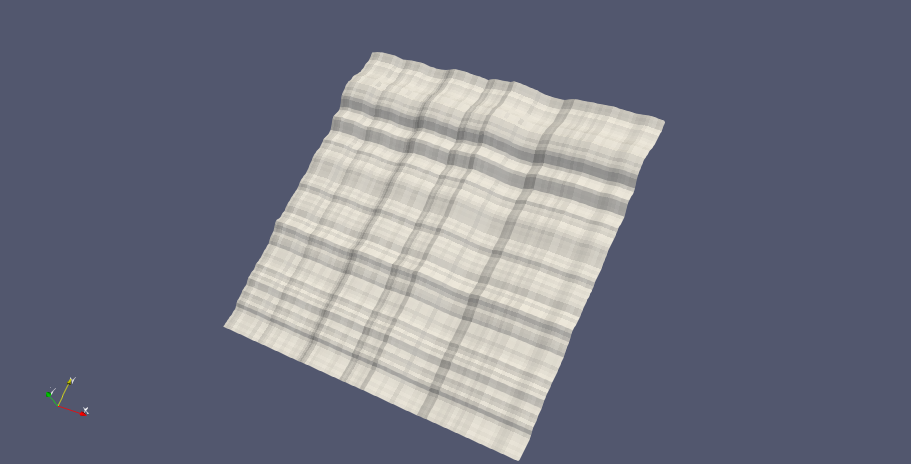
\includegraphics[width=0.7\textwidth]{caso_base_triangulacion.png}
    \caption{Malla base sin deformar.}
\end{figure}

\begin{figure}[h]
    \centering
    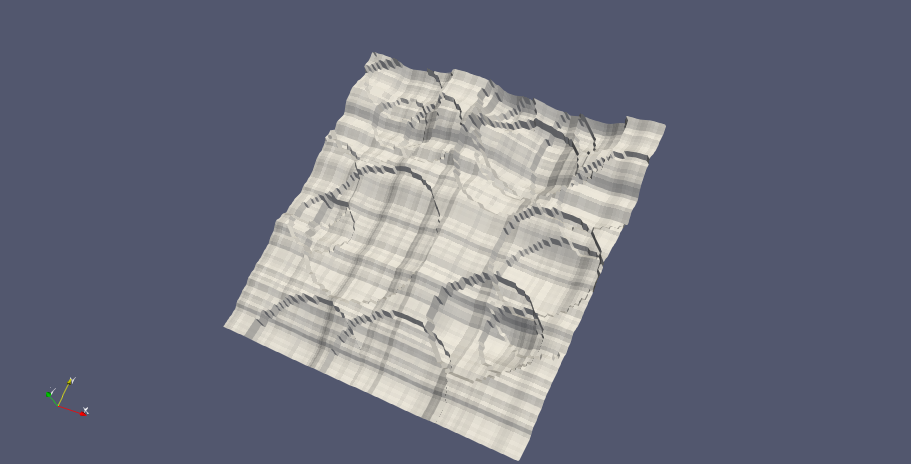
\includegraphics[width=0.45\textwidth]{gaussiana.png}
    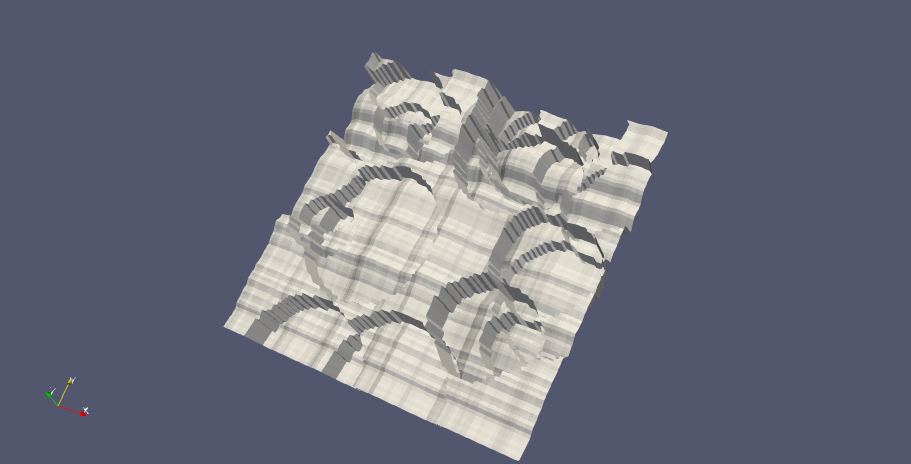
\includegraphics[width=0.45\textwidth]{multicuadrática.png}
    \caption{Resultados con función gaussiana (izquierda) y multicuádrica (derecha).}
\end{figure}

\begin{figure}[h]
    \centering
    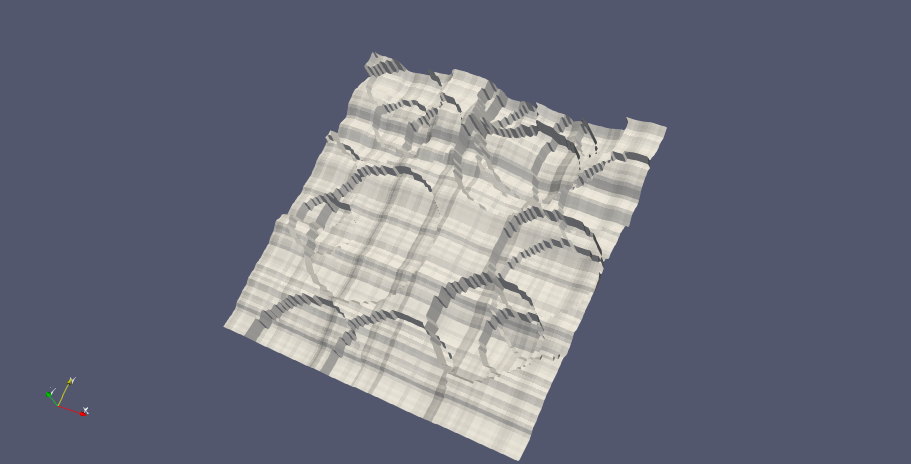
\includegraphics[width=0.45\textwidth]{multicuadrática_inversa.png}
    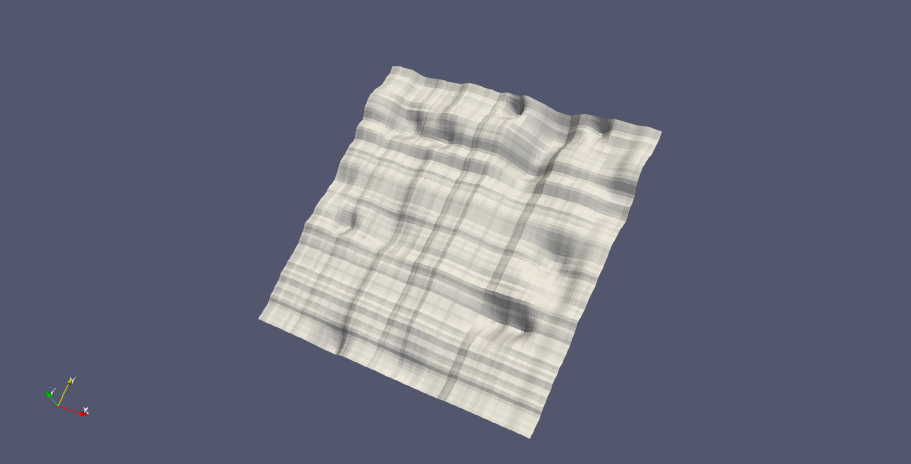
\includegraphics[width=0.45\textwidth]{wendland.png}
    \caption{Resultados con función multicuádrica inversa (izquierda) y Wendland \(\phi_{3,1}\) (derecha).}
\end{figure}

\end{document}